%\documentclass{unmeereport}
%\documentclass[final]{eeceTR} - using the final option changes layout
\documentclass[botnum, nobox]{unmeethesis}

% TODO Numbering starts on first chapter. Should be roman numerals before that, not required.

\usepackage{multirow}  % for the table
\usepackage{relsize}
\usepackage{graphicx}

\begin{document}

\frontmatter

% Uncomment the next command if you see weird paragraph spacing:
% That is, if you see paragraphs float with lots of white space
% in between them:
% \setlength{\parskip}{0.30cm}


\title{Mesh Addition Based on the Depth Image (MABDI)}

\author{Lucas E. Chavez}

\degreesubject{B.S., Mechanical Engineering}

\degree{Master of Science \\ Mechanical Engineering}

\documenttype{Thesis}

\previousdegrees{B.S., Mechanical Engineering \\
New Mexico Institute of Mining and Technology, 2009}

\date{December, 2016}

\maketitle

% \begin{dedication}
%    To my parents, Albert II and Gladys, for their support,
%    encouragement and the Corvette they're giving me for graduation. \\[3ex]
%    ``A bird in hand is worth two in the bush''
%          -- Anonymous
% \end{dedication}

\begin{acknowledgments}
   \vspace{1.1in}
   This work was support in part by Sandia National Laboratories under Purchase Order: 1179196 and  NSF grant OISE \#1131305.
\end{acknowledgments}

\maketitleabstract %(required even though there's no abstract title anymore)

\begin{abstract}
  Many robotic applications, especially those whose goal is to aid or assist
  through human-robot interaction, utilize a rich map of the world for reasoning
  tasks such as collision detection, path planning, or object recognition. Such
  map, and the method used to produce it, must take into consideration real-world
  constraints. Most mesh-based mapping algorithms resemble a ``black box'' and do
  not provide a mechanism to close the loop and make decisions about the
  incoming information. MABDI leverages the global mesh by finding the difference
  between what we expect to see and what we are actually seeing, and using this to
  classify the incoming measurements as novel or not. This allows the surface
  reconstruction method to be run only on data that has not yet been represented in
  the global mesh. The result is an algorithm that becomes computationally
  inexpensive once the environment is known, but can also react to new objects.
\clearpage %(required for 1-page abstract)
\end{abstract}

\tableofcontents
\pagebreak

\mainmatter


\section{Introduction} \label{sec:introduction}

Many robotic applications, especially those that involve human-robot
interaction, often require a rich representation of the environment in order to
perform such behavior as path planning and obstacle avoidance. In general, a
rich representation, or map, is useful for providing situational awareness to an
autonomous agent. A map is also important for applications such as teleoperation
\cite{Kadous2006}.

The methodology to build this representation is a continuously evolving subject
in the field of robotics. The origins of the research into this problem date
back roughly 25 years \cite{Lorensen1987}. Since then the methods and the
representations themselves have continued to evolve at an impressive rate. The
main catalyst behind this growth is the advancement of sensing technologies over
the same time period. In general, sensors have continued to generate
measurements at higher rates, higher resolution, and lower cost over the years.
This has provided an amazing opportunity to build richer and more useful
representations of the environment.

In robotics, map building in an unknown environment is referred to as the
Simultaneous Localization and Mapping (SLAM) problem \cite{Thrun2002}. This
label describes the fact that a methodology which solves the SLAM problem must
simultaneously locate the robot in the environment as well as map the
environment. The focus of this work is the mapping aspect of the SLAM problem.
Fig. \ref{fig:goal} gives a visualization of the goal.

\begin{figure}[h]%[thpb]
\centering
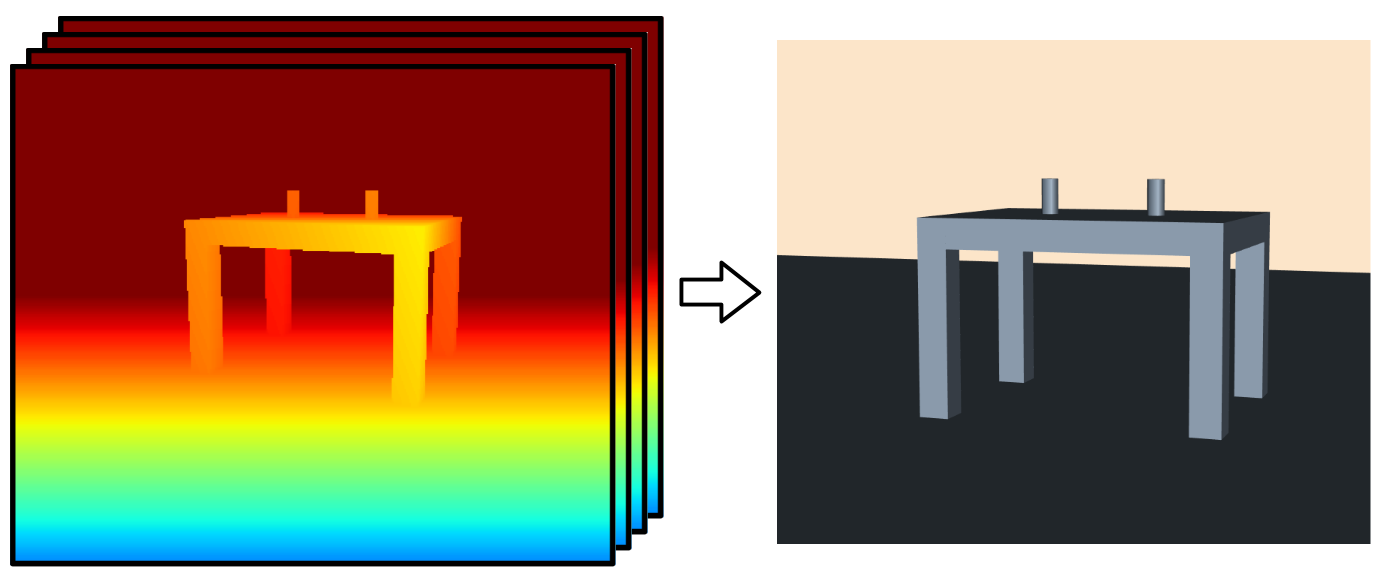
\includegraphics[width=.5\textwidth]{figures/diagram_goal.png}
\caption{Goal is to create a map from depth images}
\label{fig:goal}
\end{figure}

There are different types of data structures that can define a map. All types have both
intrinsic characteristics that impact the algorithms that generate them and
constraints that must be considered for real-world applications. In
addition, we are concerned with rich representation types, in contrast to sparse
representation types \cite{Dissanayake2001}, because rich types have the most
use in applications such as human robot interaction.

\begin{table}[h]
  \caption{Comparison of constraints for different map types}
  \label{tab:rep}
  \begin{footnotesize}
  \begin{center}
    \begin{tabular}{|l|c|c|c|c|c|}
    \hline
    \multirow{2}{*}{} & Supported & Computationally & Low Memory \\
     & & Inexpensive & Requirement \\\hline
    Point Clouds		& x & x & - \\
    Surfels             	& - & x & x \\
    Implicit Functions 	& x & - & - \\
    Mesh	 	& x & x & x \\
    \hline
    \end{tabular}
  \end{center}
  \end{footnotesize}
\end{table}

When considering what type of map is best for real-world applications, we must
consider the constraints imposed by each type:

\begin{itemize}
  \item Supported - Is there software, tools, research, algorithms, etc., for
  this type of map?
  \item Computationally Inexpensive - Can the algorithms run quickly on low cost
  computers (rather than specialized hardware)?
  \item Low Memory Requirement - Can the algorithms run on hardware with
  a standard amount of RAM?
\end{itemize}

Table \ref{tab:rep} compares the constraints of common map types. We can see, in
general a mesh type map satisfies real-world constraints. It has been used
extensively by the gaming and graphics communities, and so benefits from an
incredible amount of continued research and advances in hardware such as
Graphics Processing Units (GPUs).

Currently, one of the issues with mesh mapping techniques is they are generally
``black box'' methods. Meaning the data comes in from the sensor, those
measurements are turned into a mesh, and then that mesh is appended to a global
mesh. Fig. \ref{fig:pipeline} visualizes this common pipeline in black. The goal
of this work is to design an algorithm to close the loop (as visualized in red)
and allow the system to make decisions about the incoming data based on what it
already knows.

\begin{figure}[h]%[thpb]
\centering
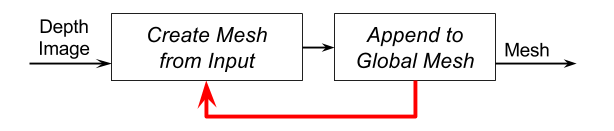
\includegraphics[width=.5\textwidth]{figures/diagram_general_pipeline.png}
\caption{Common ``black box'' pipeline in black. The contribution of MABDI in red.}
\label{fig:pipeline}
\end{figure}

% set up what environmental mapping is, what a mesh is
% design goals of the system

\section{Related Works}	\label{sec:related_works}

% Works related to MABDI are generally based on RGB-D sensors. This type of sensor has
% become very popular since the release of the Kinect from Microsoft, which
% was the first mass produced RGB-D sensor of its kind. RGB-D sensors are
% inexpensive and produce noisy 640x480 depth images at 30fps. The RGB-D
% sensor has excited the robotics community because this has been the first
% time that depth data has been so readily accessible from such an
% inexpensive sensor. Therefore, methodologies that use RGB-D data must be able to quickly
% deal with very high rates of information.
%
% Research and development of new mapping algorithms trend towards
% leveraging the information in the global map to make decisions about the
% incoming data. One can see parallels with how we as humans see the world. MABDI
% proposes do this in a computationally feasible way by simply using
% differencing and thresholding imaging methods.


A major problem in robotics has been and continues to be: How can we create
the ``best'' representation of an unknown environment? There are two main
communities of researchers who been working on developing algorithms
and methods to answer precisely this question. They are the robotics
community and the computer graphics community and each community has a
slightly different motivation for solving this problem. The robotics
community is concerned with developing a real-time solution of generating
representations in large environments. These representations are used by
both fully autonomous and teleoperated systems. The common name which is
used by the robotics community for this problem is Simultaneous
Localization and Mapping or SLAM. The name SLAM refers to the problem of
mapping and locating a robot in an unknown environment. Early methods
generated very sparse representations of the world, as time and sensor
technology progressed the representations became denser. A dense
representation is desired for any system which must have good situational
awareness of its environment. The computer graphics community is concerned
with generating high quality representations of smaller environments and
single objects. They generally refer to the problem as surface
reconstruction. These representations are used by augmented reality,
computer game object creation, 3D printing, and more applications. In the following
sections we will trace the development of representation generating methods
in both communities. We will then discuss what is needed in future work.

\subsection{SLAM}

The problem of SLAM has been a primary focus of the robotics community for
more than 25 years. A complete solution to the SLAM problem must be able to
generate a representation of an unknown environment and track the robot in
this new representation. In this body of literature the act of generating a
representation is referred to as mapping. A good overview of the problem
can be found in \cite{Durrant-Whyte2006} and \cite{Bailey2006}. Each
solution is designed to consider the goal application, type of sensor,
computational constraints, and memory limits. All these factors influence
the researcher's choice of what type of representation to use for the
mapping procedure. In 2002 Thrun wrote a famous survey \cite{Thrun2002} of
the SLAM literature which categorized existing algorithms on many traits
including the representation. The representation choice of prior work can
be roughly categorized into 3 types. The first type is characterized by
some sort of list of 2D or 3D points and are usually considered to be
sparse representations. Common names for these types are landmark locations
and point clouds. The second type are considered to be more volumetric
based and are often times considered to be a dense representation. Common
names for these types are occupancy grid and Truncated Signed Distance
Function (TSDF). The last type have the characteristic of being a surface
representation and are also considered to be a dense representation. Common
names for these types are surfels and mesh. In the following sections we
will trace the history of each of the 3 types of representation that is
seen in the SLAM literature.

\subsubsection{Point Locations}

One of the most well known and earliest solution to the SLAM problem, which
uses a point location representation, was proposed by Smith et al. in 1990
\cite{Smith1990}. The mathematical framework that he created was the origin
of a family of solutions based on the Extended Kalman Filter (EKF). The
representation he chose was simply a list of 2D landmark locations. Each
location was part of a state matrix which was estimated at every iteration.
A list of landmark locations was chosen because it allowed the method to
have a low computational cost and use a small amount of memory, important
factors in the days of early computing. There have been many improvements
to the family of SLAM solutions which generate a list of point locations
since Smith's work. One of the first practical implementations on a real
robot was done by Thrun in 1998 \cite{Thrun1998}. In this work the SLAM
problem was posed in an Expectation Maximization (EM) framework which is
similar to the EKF framework in that landmark locations are saved
in a state vector which is estimated at every iteration. In Thrun's work an
occupancy grid map is generated as a post processing step from sonar
measurements. The results showed that their representation could become
more accurate over time by using new observations to improve the current
estimate. This a highly desired ability of any representation generation
method. The next step was the ability of these methods to include a loop
closure procedure. A loop closure procedure was proposed by Gutmann in 1999
\cite{Gutmann1999}. The key ability of the method was it could recognize
when the robot was revisiting a prior location and adjust the entire
representation with the constraint that the two points must coincide. In
2001 Dissanayake et al. \cite{Dissanayake2001} derived 3 theorems to
theoretically prove the convergence of the SLAM problem. Their test
platform used a millimeter-wave radar mounted on a vehicle and generated a
list of 2D landmark locations. In 2001 Thrun et al. \cite{Thrun2001} cast
the SLAM problem using particle filter techniques. Their results generated
a 2D map and showed an increased robustness and lower computational cost
than prior methods. One of the key disadvantages of methods up to this
point was that complexity scaled quadratically with the number of landmark
locations.  In 2002 Montemerlo et al. \cite{Montemerlo2002} created a SLAM
solution named FastSLAM which was able to handle a much larger number of
landmarks. They showed results with maps containing more than 50,000
points. Then, SLAM solutions using point locations became much more
directed towards 3D.

Some of the first interesting works which represented the world as a list
of 3D point locations were done by Thrun et al. in 2000 \cite{Thrun2000},
Liu and Emery in 2001 \cite{Liu2001}, and H\"{a}hnel et al. in 2003. In
these works the 2D landmark locations and robot position were estimated
using very similar techniques from past work. Once this had been done the 3D
laser scan data was simply appended to each estimated robot location. Then,
a mesh was created by post processing the 3D point cloud. They utilized the
fact that the laser collected the data in an incremental manner and simply
connected neighboring 3D points. Finally, the mesh was simplified by
looking for large planar sections and merging the corresponding mesh
elements. One of the first SLAM solutions which used a single camera to
generate a list of 3D points was done by Davison in 2003
\cite{Davison2003}. Here he used a single camera to generate a very sparse
list of 3D points. This method was limited to small environments. Future
advances allowed representations of larger environments. In 2003 Thrun et
al.  \cite{Thrun2003} created a SLAM procedure which did not rely on having
a structured environment and was applied to mapping large mines. In 2004
Howard et al. \cite{Howard2004} created a SLAM systems based on a Segway
platform equipped with a 3D laser which could map large areas of roughly 0.5
km on each side.  One of the results showed a map with approximately 8
million points. In 2006 Cole and Newman \cite{Cole2006} continued work in
large-scale SLAM by increasing robustness and also generated maps with many
3D points using a laser sensor. In 2007 Clemente et al. created a
large-scale SLAM system that used a single camera. The system had an
advanced loop closing procedure based on visual features and created large
maps of 3D points. In 2001 Klein and Murray \cite{Klein2007} developed a
SLAM solution which used a single camera. The uniqueness of their
method was the algorithmic structure. Their SLAM solution consisted of 2
separate processes: a tracking processes and a map building process. This
algorithmic structure has become very common in many current SLAM solutions
because of the advances in pose estimation technology. Klein and Murray
were able to get very good results for a small environment and showed
Augmented Reality (AR) applications.  Many of the future advances of SLAM
solutions, which generated 3D point sets, dealt with camera systems
\cite{Paz2008,Konolige2008,Strasdat2010} and improved in speed and
robustness. Many of the most current methods which produce a list of points
are systems that use a relatively new type of sensor named a RGB-D sensor.
One good example is a work that was produced in 2011 by Engelhard et al.
\cite{Engelhard2011}. In this work they used an algorithm named the
Iterative Closest Point (ICP) \cite{Rusinkiewicz} to align point clouds
from coming from the RGB-D sensor into a large colored point cloud.  The
resulting maps were visually impressive. However, the map could not be
adapted to new information and was not well suited for other applications,
such as obstacle avoidance. These limitations are inherent in maps that
consist of lists of points.

\subsubsection{Volumetric}

Many SLAM solutions generate a 2D volumetric representation of the world
because they are especially advantageous in dealing with noisy sensors. Two
of the first major works which generated a 2D volumetric representation
were done in 1998 by Yamauchi et al. \cite{Yamauchi1998} and Schultz et al.
\cite{Schultz1998}. These works generated a 2D occupancy grid which is a
type of volumetric representation. Here the environment was divided into a
2D grid.  Each square of the grid contained the probability that it was
occupied with an object. All squares would be updated iteratively based on
the current sensor readings. Occupancy grids, like any other
volumetric-based representation, are limited by the amount of available
memory. In 2002 Biswas et al. \cite{Biswas2002} extended occupancy grid
methods by allowing dynamic environments. This was done by looking at past
``snapshots'' of the map. In 2004 Eliazar and Parr \cite{Eliazar2004}
continued the advancement by decreasing computational cost and implemented
a loop closure method.

There have been a few impressive SLAM solutions which generate a 3D
volumetric representation. There are three major works which generated
something very similar to a 3D occupancy grid which was saved as in a
octree data structure
\cite{Magnusson2007,Nuchter2007,Huang2011,Endres2012}. Each work had a
slightly different name and procedure for generating the representation,
but in general the representations divided the environment into cubes and
had a scalar value representing the belief of a surface being there.
Octrees were used to save memory by only having a fine resolution of cubes
at places where there was a surface. There are many advantages to a 3D
occupancy grid representation. When applied to obstacle avoidance and path
planning algorithms. Also, the representation is very adaptable to new
information. The major disadvantage is that the representation can not be
visualized immediately. In order to render, an image must be generated at
each desired viewpoint by ray tracing the volume. This can be a problem
when using such method for applications such as teleoperation due to the
computational cost of rendering. The current state of the art for
generating a volumetric representation was done by Newcombe et al.  in 2011
\cite{Newcombe2011a}.  Their system used a RGB-D sensor and generated a 3D
voxelized grid Truncated Signed Distance Function (TSDF) of the
environment. For this type of representation each cube contains the value
of the distance to the nearest surface. The sign of the value is based on
which side of the surface the cube is relative to the sensor. This work has
been the most capable at dealing with extremely noisy data and dynamic
scenes. However, due to memory constraints the method can only represent
environments that are about the size of a 4m cube. Also, it must be ray
traced in order to be visualized.

\subsubsection{Surface}

One of the first major works which created a surface representation of the
environment in real-time was done by Martin and Thrun in 2002
\cite{Martin2002}. Their method utilized an EM framework to fit plane
models to 3D point cloud data. Polygon mesh elements were then easily
assigned to each plane. The main drive behind this work was to generate a
map of the environment that uses a low amount of memory. Their  method
worked well for structured environments. One of the major limitations of
their method, and other methods that only mesh large planar sections, is
that the representation will only consist of planar sections and not
capture the fine detail of the environment. In 2004 Viejo and Cazorla
\cite{springerlink:10.1007/978-3-540-30463-0_30} developed a methodology
for generating a mesh that can contain more information of the environment
than large planar sections. Due to this ability, they termed their method
to be ``unconstrained.'' Essentially their method was based on a 3D
Delaunay triangulation algorithm. Giesen surveyed Delaunay triangulation
methods in \cite{Giesen2004}. Viejo and Cazorla were not able to obtain
real-time results and, in fact, it has been seen that it is extremely
difficult to run a 3D Delaunay triangulation in real time because of the
numerous amount of distance calculations that are needed.  One of the next
major advances came from Weingarten and Siegwart in 2006
\cite{Weingarten2006}. Their work also created a mesh that was only capable
of capturing large planar surfaces. However, they showed increased
robustness. In 2007 Pollefeys et al. published a work with multiple
researchers \cite{Akbarzadeh2006,Pollefeys2007}. They developed a large
urban mapping system consisting of a vehicle and eight camera systems. The
processing was carried out by multiple CPUs and optimized with Graphics
Processing Unit (GPU) calculations. In their work they used the camera
systems to generate depth maps. The set of depth maps was then fused to
create a new smaller set of depth maps that were more accurate. The depth
maps in the smaller set were more accurate because the error was averaged
out by using near-by depth maps. The smaller set was then used by a
triangulation procedure to create a mesh of the environment.  The mesh
generation procedure was based on a work from 2002 by Pajarola et al.
\cite{Pajarola2002}. This method defines a mesh in the depth image. It
starts from a very coarse mesh and continues to refine in areas of the
depth image based on a confidence criteria. In the work of Weingarten and
Siegwart these meshes which are defined for each fused depth image are then
checked for overlaps and duplicates are removed to make a single large
mesh. One of the major drawbacks of this approach is that the output mesh
can not be adapted by measurements which come from revisited parts of the
scene. Another major advancement came in 2008 from Poppinga et al.
\cite{Poppinga2008}. In this work they used a Time of Flight (ToF) camera
to generate a mesh representation of the large planar structures in the
environment. Here they also develop a procedure to determine a mesh in a
depth image. They leverage the structure of the depth image to make the
method computationally inexpensive. In their work they simply append the
meshes which are created from each depth image into a global coordinate
system. They obtain very good results from a simple method.  Once
again, the method is not adaptive to new information. Also, a mesh is
created for each depth image instead of updating and maintaining a global
mesh. A major advancement came from a famous work done by Newcombe and
Davison in 2010 \cite{Newcombe2010}. In this work they designed a method to
create a mesh reconstruction from a single video camera. Their method used
Structure From Motion (SFM) to obtain a sparse point cloud of the scene.
Then an implicit function was fit to the point cloud using the methodology
of Ohtake et al.  \cite{Ohtake2003}. A bundle of depth maps is then
selected. From the bundle a single reference depth image is selected and a
``base'' model is constructed by sampling the implicit surface for vertices
in the reference frame. The neighboring frames are used to better the
``base'' model and create a more accurate mesh. Each reference frame has
its own mesh and all the meshes are put into a global coordinate system.
Duplications are then detected and removed. Again, the representation is
not adaptive to new information. In 2010 St\"{u}hmer et al.
\cite{Stuhmer2010} advanced the field by publishing a method to generate
very accurate depth maps from several color images in real-time. They
showed very impressive results but their method was not designed to maintain
a representation in a global coordinate frame.

The next major advances in methods that generated surface representations of the
environment, were based on RGB-D sensors.This type of sensor has become very
popular since the release of the Kinect from Microsoft which was the first mass
produced RGB-D sensor of its kind. RGB-D sensors are inexpensive and produce
noisy 640x480 depth images at 30Hz. The RGB-D sensor has excited the robotics
community because this has been the first time that depth data has been so
readily accessible from such an inexpensive sensor. Therefore, these
methodologies must be able to quickly deal with very high rates of information.
One impressive work came from Henry et al. in 2012 \cite{Henry2012}. In this
work they designed a system which used a RGB-D sensor to build a map made of
surfels (Surfels are circular disks which have a particular position and
orientation and also a radial size based on confidence.). In order to generate
and maintain the surfel map they used the work of Weise et al. \cite{Weise2009}.
The map consists of a large number of surfels. The surfel map can be updated
given new registered depth images from the sensor. Decisions are made how to
handle each measurement in the depth image based on the difference between an
expectation generated using the current map and the actual readings from the
sensor. Rendering a surfel map requires special methods \cite{Pfister2000} and
is difficult to use in applications such as obstacle avoidance.

One of the next major advances is a highly-related work that was published by
Whelan et al. in 2012 \cite{Whelan2012} and more recently in 2013
\cite{Whelan12tr}. The system they developed was named Kintinuous and was able
to produce a high quality mesh representation of the environment. Their hybrid
system utilized the KinectFusion method \cite{Newcombe2011a} of Newcombe et al.
to create a volumetric representation of the portion of the environment in front
of the sensor. As the sensor moves, portions of the environment that leave the
volume in front of the sensor are ray cast and turned into a mesh. They obtain
very impressive results but also mention a limitation of their system for future
work. The limitation is that the mesh can not be updated once created, which is
an issue when revisiting parts of the environment. One of the most impressive
current works which has an adaptable mesh came from Cashier et al. in 2012
\cite{Cahier2012}. In this work, they were able to generate and update a mesh
with new measurements from a ToF sensor. They used the difference between the
existing model and the actual measurements to decide whether to adapt the mesh
or add new elements. The mesh topology was not adaptive to the environment and
their experiments only showed results of mapping a single flat wall with no
robot movement. The system needs to be tested for object addition and removal.

\subsection{Surface Reconstruction}

The computer graphics field has spent considerable effort to develop methodologies
for creating representations from sets of data. Generally, these sets of
data are acquired from a sensor. Methodologies have progressed steadily and
are often designed for a specific application. One of the original motivations
was to generate surfaces from medical imaging data. This
allows doctors to make better decisions because the data are presented in a
more intuitive manner. Current applications include augmented reality and
3D printing. Older methodologies were not as concerned with speed and often
times had a large computational cost. Also, the methodologies are often
designed for single objects or small environments. Following the taxonomy
of such well-known works as \cite{Gopi2002,Mencl1997}, the field can be
roughly divided into representations that are generated with volume-based
techniques and those that use surface-based techniques. Methods that use
volume-based techniques are characterized by spatially subdividing the
environmental volume and are usually computationally expensive and require
a large amount of memory. Methods that use surface-based techniques
generate the representation using surface properties of the input data.
Both types of methods can have mechanisms to adapt the mesh to noisy or new
information.  In the following section we will trace the progression of the
methodologies.

\subsubsection{Volume-based}

Volume-based methods spatially subdivide the volume into smaller parts and
operations are performed on the mesh to either implicitly imply the surface
or define the surface depending on the information contained in each
subdivision. One of the first well-known works that used a volume-based
technique was proposed by Lorensen and Cline in 1987 \cite{Lorensen1987}.
In this work they proposed a method named marching cubes which is still
known for its reliability and simplicity and is used by applications which
do not have a computational requirement. Marching cubes subdivides the
space into cubes. The data contained in each cube dictate how the surface
connectivity will be defined in that cube. Possible vertex locations are at
the corners and along the edges. Once this has been done for all cubes the
process is complete. One of the next major steps came from Hoppe et al. in
1992 \cite{Hoppe1992} In this work they used the input points to define a
Signed Distance Function (SDF) in 3D space and then meshed the zero-set to
obtain the output mesh. A SDF is a spatial function which has the value of
the distance to the nearest surface at each point. The sign is used to
specify if the point is inside our outside of the surface relative to the
sensor. The zero-set of the SDF is the surface where the values transition
from positive to negative. Using a SDF has proven to be very effective and
has been the core idea of many methodologies that came after this work of
Hoppe et al., such as KinectFusion \cite{Newcombe2011a}. One of the next
advances came from Edelsbrunner and M\"{u}cke in 1994
\cite{Edelsbrunner1994} with a method named alpha shapes. Here they used 3D
Delaunay triangulation and the input point set to decompose the volume into
a Delaunay tetrahedrization. This gives a triangulation of the input set
which involves all points. A sphere of radius alpha is then used to remove
edges and vertices to obtain a mesh of user specified resolution. Many
works have made use of 3D Delaunay triangulation to create a mesh. Methods
which use 3D Delaunay on the input set have a large computational cost and
often cannot be executed in real-time.  The next valuable contribution came
from Bloomenthal in 1994 \cite{Bloomenthal1994} as open source software for
surface polygonization of implicit functions. This was a stable and robust
open source software that has been used in many well-known algorithms
\cite{Newcombe2010}.  Another major advance came from Curless and Levoy in
1996 \cite{Curless1996}. In this work they also constructed a Truncated
Signed Distance Function (TSDF). A TSDF is very similar to a SDF, the only
difference is that distance values are truncated after they exceed a
certain threshold. Their method was one of the first to be able to handle
several registered range scans.  Their work showed how well a TSDF can deal
with several noisy scans by naturally integrating out the error. They
obtained very good results but not even close to real-time. A speed up in
processing time was achieved by Pulli et al. in 1997 \cite{Pulli1997} by
utilizing octrees. They obtained good results and their method was used by
Surmann et al. \cite{Surmann2003} in a well-known robotic mapping work.
Another major advance came in 2001 from Zhao et al \cite{Zhao2001}. They
used Partial Differential Equation (PDE) methods to obtain a final
reconstruction that was of better quality than prior methods. In 2001 Carr
et al. \cite{Carr2001} created a volumetric method based on the radial
basis function (RBF). Their method was able to successfully deal with holes
and generate water tight models. A water tight model is useful for single
object reconstruction. However, it is not desired for mapping large
environments. One of the next major advances was published in 2003 by
Ohtake et al. \cite{Ohtake2003}. In this work they created a method which
was faster than the work of Carr et al.  \cite{Carr2001} by implementing a
hierarchical approach with compactly supported basis functions. Their work
has been considered to be the state of the art for calculating an implicit
function of a noisy point set and was used by Newcombe et al.
\cite{Newcombe2010}. Volume-based methods have been able to create high
quality representations and work well for single objects and small
environments. These methods must spatially divide the environmental volume
and therefore have a high memory requirement.

\subsubsection{Surface-based}

One of the first interesting and adaptive surface-based methods was
published by Terzopoulos and Vasilescu in 1991 \cite{Terzopoulos1991a} and
dealt with 2.5D data such as intensity and range images. The goal of their
work was to create an adaptive mesh of an input image. The mesh was
initialized as a 2D sheet of mesh elements with virtual springs along each
edge. The stiffnesses of the virtual springs would then adjust based on the
image information at that location. The mesh was able to adapt to be more
dense in regions of higher intensity. In 1992 Terzopoulos and Vasilescu
extended their methodology to 3D data \cite{Vasilescu1992}. In this work
they used the distance between the mesh and the data to drive the vertices
to be near the surface. In this early work they needed to initialize the
mesh and control the subdivision of mesh elements to obtain a suitable
resolution. In 1993 Hoppe et al. \cite{Hoppe:1993:MO:166117.166119}
published a method to optimize to resolution of a given mesh by posing the
problem in an energy minimization framework. They minimized an energy
function which tried to adequately represent the surface in the most
concise mesh possible. One of the next advances in physical based
adaptation of meshes came in 1993 from Huang and Goldof \cite{Huang1993}.
In this work they were able to adjust the size of the mesh elements to
obtain a better resolution in areas of high frequency information using a
physical based model. In addition, it was one of the first works to
represent an object undergoing deformation. They method was able to perform
tracking on simple simulation examples. Another advancement came in 1994
Rutishauser et al. \cite{Rutishauser1994} with a method specifically
designed for incremental data. Their methodology worked with a sequential
input set of range data and used a probabilistic framework to adjust the
vertices of a mesh to the expected value given the prior observations.
Their methodology also modeled the noise of the sensor with a sensor model.
In 1994 Delingette \cite{Delingette1994} developed a methodology to
generate a simplex mesh model of structured and unstructured 3D datasets.
Elastic behavior of the mesh surface was modeled by local stabilizing
functionals. Also, they implemented an iterative refinement process to
refine the mesh in areas of high frequency information. One of the next
steps was published by Turk and Levoy in 1994 \cite{Turk1994}. Their method
allowed overlapping meshes to be ``zippered'' into a single mesh surface.
This ability is especially important for methods that generate a mesh for
each depth image of the sensor and then need to combine all registered
meshes into a single mesh. Their method is computationally expensive due to
distance calculations. An interesting work came in 1995 from Chen and
Medioni \cite{Chen1995}. They devised an adaptive mesh methodology based
on the inflation of a balloon. A mesh sphere was first initialized within
the registered range measurements of the object. Virtual inflation forces
were then used to expand the balloon until the mesh surface was a minimal
distance from the range data. This method was limited to objects which are
water tight. A major advancement came in 1999 from Bernardini et al.,
\cite{Bernardini1999a} in a method named the ball-pivoting algorithm. Their
method is a good example of an advancing front method. These types of
algorithms start with a seed mesh element and advance the boundary by
adding new mesh elements in the immediate area of the boundary which is
supported by measurements. Most advancing front algorithms differ in how it
is decided to add new mesh elements. In the work of Bernardini et al. a
virtual sphere of a user defined radius is rolled along the boundary of the
mesh and new elements are added if the ball touches another measurement.
Their methodology became popular because of its simplicity. One major
disadvantage was that the generated mesh was a fixed topology. Another
advancing front method came in 2001 from Gopi et al.
\cite{Gopi2001,Gopi2002}. Here they sampled the input dataset to obtain a new
dataset with a lower density of points in areas of lower frequency
information. This effectively gave their method an adaptive topology. Next,
a local neighborhood was computed at each data point and projected to a
plane tangent to the surface. The triangulation is then computed on this
local tangent plane. They obtained impressive results on datasets of
varying sample density and curvature. An interesting work was published in
2003 by Ivrissimtzis et al. \cite{Ivrissimtzis2003}. Here they used a
neural network model to adapt a mesh model to the data. They claimed that
their method is computationally independent of the size of the input
dataset because the dataset is only sampled by the method. There obtained
good results. In 2004 Alexa et al. published a very interesting
work to generate point set surfaces from an input dataset \cite{Alexa2004}.
They use moving least squares (MLS) to locally approximate the surface with
polynomials. The original dataset is then no longer used. Instead, they
develop tools to sample the approximated surface to any resolution desired
so that the end result is another point set of user specified resolution
lying closer to the surface than the input dataset. One drawback is they
had to develop their own methodology to render a point set. In 2005
Scheidegger et al. used the work of Alexa et al. to develop an advancing
front methodology to generate concise meshes of high accuracy. Their main
contribution was to augment an advancing front algorithm with global
information so that the triangle size could adapt gracefully to any change.
They obtained very impressive results. Most methodologies in Surface
Reconstruction had been solely concerned with object or small environment
recreation and have computational or memory requirements which do not work
well with large environments. One of the first successful methods intended
for large environments was published in 2009 by Marton et al.
\cite{Marton2009}. Their methodology was an advancing front algorithm which
worked on a point set which was sampled from the MLS surface of the
original point set. They were able to obtain impressive and near real-time
results on datasets of large environments. They also developed a method to
deal with revisited parts of the scene by determining the overlapping area
and reconstructing only the updated part of the surface mesh. While this is a
step forward, it would be better if the mesh surface converged
to the actual surface with an increasing number of measurements. To support
dynamic scenes they developed mechanisms to decouple and reconstruct the
mesh quickly. They only discussed these mechanisms in theory and had no
results of how these mechanisms work. While Surface-based Surface Reconstruction
techniques have developed impressively, several key issues arise
when applying these techniques to mapping large environments.

\subsection{Summary}

The fields of Robotics and Computer Vision have developed many exciting
methodologies to construct representations from a noisy input dataset.
However there is still work to be done to obtain the ideal reconstruction
method. A mesh is clearly a desirable type of representation and an
efficient method should be able to generate and maintain a mesh
representation. Also, many existing methods do not leverage the inherent
structural information contained within the depth image. There are imaging
processing techniques that could be used to answer some of the remaining
problems in surface reconstruction, such as the need for adaptive topology
and the need to decide how each measurement should be used to update the
existing mesh. Henry et al. \cite{Henry2012} has already investigated using
the difference between the expected and actual measurements to guide the
decision of how to use each measurement. However, their work was intended
for surfels and needs to be extended to meshes. A method to generate a
representation is needed which is computationally and memory efficient and
can better adapt the representation to new information.

% show many mesh based algorithms are black box
% systems capable of introspection such as kinectfusion rely on volumetric
% representation and are computationally and memory expensive

\section{Approach}	\label{sec:approach}

The algorithmic structure of MABDI can be seen in Fig. \ref{fig:system}. The
diagram is very similar to Fig. \ref{fig:pipeline} with the exception of the
Classification component, shown in blue. This Classification component is
MABDI's contribution to the state-of-art in mesh based mapping algorithms, and
is what gives MABDI the ability to make decisions about the incoming data.

The Classification component consists of two elements:
\begin{enumerate}
    \item \textit{Generate Expected Depth Image $E$} - Here we take the global
    mesh $M$, render it using computer graphics, and use the depth buffer of the
    render window to create a depth image $E$ of what we expect to see from our
    sensor. This method requires the current pose $P$ of the actual sensor
    (simulated for our experiments).
    \item \textit{Classify Depth Image $D$} - Here we classify the actual depth
    image $D$ (simulated for our experiments) by first taking the absolute
    difference between $E$ and $D$ and thresholding. If the differences are
    small, those points are thrown away and if the differences are large, those
    points are kept as $D_n$. The idea behind this is, if the difference is
    large, the measurements are coming from a part of the environment that has
    not been seen before, i.e. novel. The implication of this assumption is that
    this version of MABDI cannot handle object removal. It is worth noting
    that MABDI can be extended to handle object removal by using the sign of the
    difference between $E$ and $D$ instead of the absolute value.
\end{enumerate}

\begin{figure}[h]%[thpb]
\centering
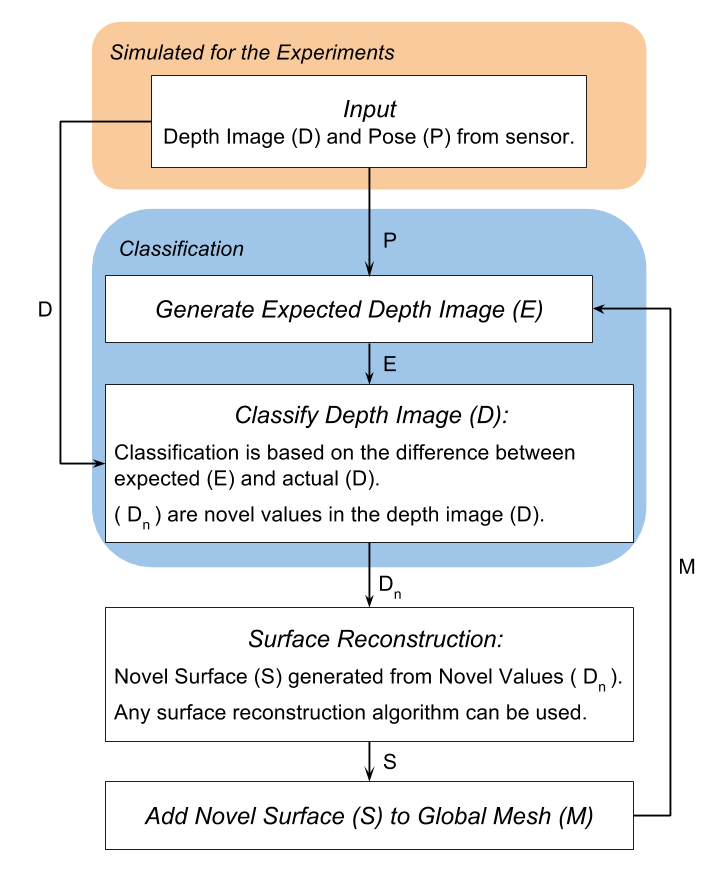
\includegraphics[width=.5\textwidth]{figures/diagram_system.png}
\caption{MABDI system diagram}
\label{fig:system}
\end{figure}

From a software perspective, the major difficulty of implementing the MABDI
algorithm was found to be creating both the simulated depth image $D$ and the
expected depth image $E$. In addition, managing the complexity of the data
pipeline needed to run the algorithm and the simulation of the sensor proved to
be difficult. Thankfully, Kitware, who is a leading
edge developer of open-source software, created the Visualization Toolkit (VTK)
\cite{schroeder2004visualization, sitevtk}. At the time of this writing the VTK
Github repository has over 60,000 commits and is contributed to by supporters
such as Sandia National Labs \cite{sitesandia}.

MABDI implemented in Python and uses VTK. The code is available upon request to
golucasplus@gmail.com. At the time of this writing, it consists of over 1,400
lines. The code that implements the MABDI algorithm itself is around 750 lines.

VTK is aptly designed for the implementation of MABDI for many reasons. Perhaps
the most important is the concept of a vtkAlgorithm (often called a Filter).
This allows a programmer to create a custom and modular processing pipeline by
defining classes that inherit vtkAlgorithm and then defining the connections
between these classes. For example, you could have a pipeline that reads an
image from a source (component 1), performs edge detection (component 2), and
then renders the image (component 3). Using this concept, the individual
elements of MABDI can be succinctly defined in individual classes. With that in
mind, we can see in Fig. \ref{fig:software} the layout used in my implementation
of MABDI. Note, vtkImageData and vtkPolyData are VTK types used to represent an
image and mesh respectively:

\begin{itemize}
    \item  \textit{Source} - Classes with the prefix Source define the
    environment that is used for the simulation and provide a mesh in the form
    of a vtkPolyData.
    \item \textit{FilterDepthImage} - Render the incoming vtkPolyData in a
    window and output the depth buffer from the window as a vtkImageData. The
    output additionally has pose information of the sensor.
    \item \textit{FilterClassifier} - Implements the true innovation of MABDI,
    takes the difference between the two incoming depth images (vtkImageData)
    and outputs a new depth image where the data that is not novel is marked to
    be thrown away.
    \item \textit{FilterDepthImageToSurface} - Performs surface reconstruction
    on the novel points. In this simple implementation the topology of the mesh
    is defined in the image coordinates and can be thought of as a checkerboard
    pattern with two triangles in every square. The data is then projected to
    real-world coordinates. The topology and the real-world coordinates are
    combined to define a surface and output as a vtkPolyData.
    \item \textit{FilterWorldMesh} - Here we simply append the incoming novel
    surface to a growing global mesh that is also output as a vtkPolyData.
\end{itemize}

\begin{figure}[h]%[thpb]
\centering
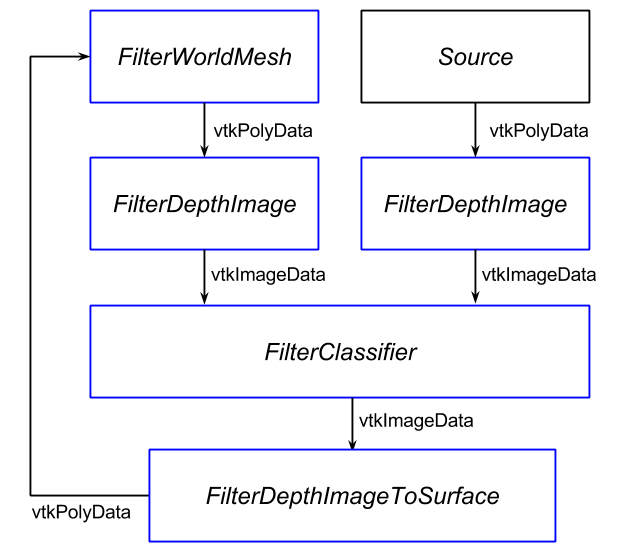
\includegraphics[width=.5\textwidth]{figures/diagram_software.png}
\caption{MABDI software diagram}
\label{fig:software}
\end{figure}

% How Mabdi works, describe the algorithm
% How Mabdi is implemented

\section{Experimental Setup}	\label{sec:experimental_setup}

It was decided to develop and test MABDI in a completely simulated environment
so that all results could be repeatable and also to facilitate the ability to
debug during the development process. This ability was truly invaluable as some
components of the algorithm proved to be complex from an implementation
perspective. In addition, we can now compare the resultant
global mesh to ground truth.

\subsection{Simulation Parameters}

The simulation was designed to be highly configurable and is implemented by a
class named MabdiSimulate. The class is initialized with parameters that control
all aspects of the simulation. Parameters of a particular importance are
discussed in more detail here:

\begin{itemize}
    \item  Environment - This parameter specifies the environment used to generate
    the simulated depth images. \textit{Table} is an environment consisting of a
    table and two cups placed on the table. The table is 1 meter tall.
    \textit{Bunnies} is an environment consisting of three bunnies who are
    around 1.5 meters tall. These bunnies are created using the Stanford Bunny
    \cite{Turk1994}, a well known data set in computer graphics.
    \item Noise - If true, adds noise to the depth image of the simulated sensor.
    \item Dynamic - If true, adds an object during the simulation. In the case
    of this analysis, a third bunny is added half-way through the simulation.
    \item Iterations - The number of iterations the simulation will have. This
    parameter affects the distance the sensor travels from frame to frame.
\end{itemize}

% parameters chosen the experimental runs
For this paper we will be exploring three experimental runs to demonstrate the
ability of the MABDI implementation to generate valid results. Additionally, the
experimental runs will be able to show the capabilities of the MABDI algorithm
such as handling object addition in the environment.

\begin{table}[h]
  \caption{Description of the experimental runs.}
  \label{tab:run}
  \begin{footnotesize}
  \begin{center}
    \begin{tabular}{|l|c|c|c|c|}
    \hline
           & Environment & Noise   & Dynamic & Iterations \\\hline
    Run 1	 & Table       & False   & False   & 30 \\
    Run 2  & Bunnies     & True    & False   & 50 \\
    Run 3  & Bunnies     & True    & True    & 50 \\
    \hline
    \end{tabular}
  \end{center}
  \end{footnotesize}
\end{table}

All experimental runs define a helical path for the sensor to follow during the
simulation. The path circles the objects in the environment twice. A helical
path was chosen because it returns to a part of the environment that has been
already mapped and is thus ``known'' to the global mesh. Also, because the path
is a helix and not just a circle, the sensor views the environment from a
slightly different position on each pass.

\subsection{Analysis of Simulated Noise}

In order to realistically simulate the sensor in a real-world environment we add
noise to the depth image $D$. See Fig. \ref{fig:system}. The magnitude of the
noise added is based on the accuracy of real-world sensors. As new RGB-D sensors
have been developed, such as the Asus Xtion and the Kinect for Xbox One, the
accuracy of the sensors has continued to improve \cite{lachat2015first}. For
this work, we take a conservative approach and utilize the well known error
modeling work of Khoshelham \cite{Khoshelham2012} that is based on the original
Kinect.

The depth image used by the MABDI algorithm $E$ and the depth image that comes
from simulating the environment $D$ both use a pinhole camera model. This method
has been validated in the localization work of Fallon \cite{Fallon2012}. The
intrinsic camera parameters of the pinhole hole model were chosen to emulate the
Kinect sensor \cite{sitekinectspecs}. The pinhole model defines a transformation
matrix used to transform between viewpoint coordinates and real-world
coordinates. The z component of the viewpoint coordinates constitutes the depth
image and are defined to vary between 0 and 1. Due to how the transformation
works, differences in the depth image do not linearly correspond to changes in
real-world coordinates as can be seen in Fig. \ref{fig:depth}.

\begin{figure}[h]%[thpb]
\centering
  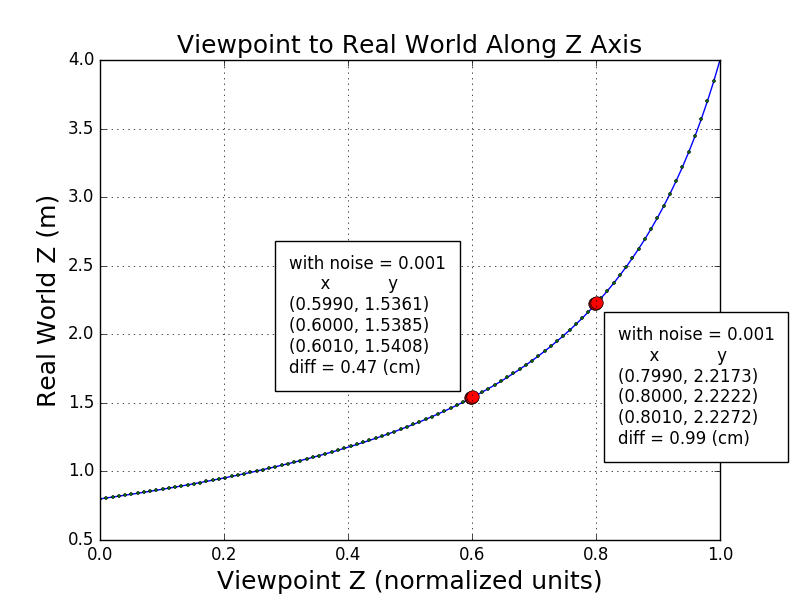
\includegraphics[width=.5\textwidth]{figures/plot_depth.png}
  \caption{Viewpoint coordinates to real world coordinates analysis.}
  \label{fig:depth}
\end{figure}

The noise added to $D$ is defined by the equation below. The standard deviation
$\sigma\mathsmaller{=}0.001$ was chosen so that the resultant errors in the
real-world coordinates would correlate to the error model in
\cite{Khoshelham2012}. The text boxes in Fig. \ref{fig:depth} show the resultant
real-world error for two values of $D$; they match the error model of
\cite{Khoshelham2012}.

$$
D_{noisy}(i,j) = D(i,j) + D(i,j)*\mathcal{N} (\mu\mathsmaller{=}0, \sigma\mathsmaller{=}0.001)
$$

% Can add equation showing addition of noise if there is space later

% Viewpoint coordinates to real-world coordinates analysis. Viewpoint coordinates
% are obtained when a mesh is rendered into a render window, and can be
% transformed to real-world coordinates using the transformation matrix of the
% camera. Noise is added in simulation to the viewpoint coordinates. This graph
% shows the effect of that noise in real-world coordinates.

% describe the simulation environment
% maybe determine speed of walker
% discuss noise

\section{Results} \label{sec:results}

% overview of runs
An overview of the experimental runs is given in Fig. \ref{fig:run123}. The figure shows a set of six views of information for each run. These views are created at every iteration and generate a movie of the run. Fig. \ref{fig:run123} shows a snapshot of these views at different points of the simulation for each run. The views are described below:

\begin{itemize}
  \item Top Left - View of the global mesh $M$ from a third perspective. The
  wire frame corresponds to the viewing frustum of the sensor. The light blue
  helical line is the path of the sensor. Gray is the simulated environment.
  The multi-colored mesh is the global mesh $M$. The mesh is multi-colored in order
  to show the passage of time. For example, in Run1, The mesh is colored yellow,
  light green, and dark green for iterations 1, 2, and 3 respectively.
  \item Top Middle - Same as Top Left except it shows the novel surface $S$ instead of
  the global mesh $M$.
  \item Top Right - Plot showing the number of elements in the global mesh $M$
  up to this iteration.
  \item Bottom Left and Bottom Middle - Actual $D$ and expected $E$ depth image
  respectively.
  \item Bottom Right - The classified depth image. Novel point $D_n$ are shown
  in black. Points to be thrown away are shown in white.
\end{itemize}

We can notice important aspects of MABDI using Fig. \ref{fig:run123}. Notes on each of the runs:

\begin{itemize}
  \item Run 1 - Top Left shows how the $M$ gets composed over time.
  It is important to note that the mesh is not overlapping itself. This can be
  understood by noticing $S$ from Top Middle is the same as
  the section of $M$ this is colored dark green.
  \item Run 2 - This run shows clearly how the classification process is able to
  distinguish novel points. This can be seen by noticing the valley in-between
  the ear and the eye of the bunny closest to the sensor. The sensor was not
  able to see these points from the prior iteration due to occlusion. From the
  sensor's current perspective, the points can now be seen. Notice how the
  valley is missing in the \emph{expected} depth image $E$, classified as novel
  in Bottom Right, and thus reconstructed into $S$. This is a clear example of
  the concept behind MABDI.
  \item Run 3 - This run shows how MABDI reacts to object addition. At this
  iteration the middle bunny is suddenly added. We can follow the data: $D$
  shows the new bunny, $E$ shows what we expect to see (the middle bunny is not
  there because it is not in $M$), Bottom Right shows all points corresponding
  to the new bunny as marked as novel, and finally the novel points are
  reconstructed as $S$ and appended to $M$. Top Right also shows a large jump in
  the number of elements in $M$ due to the new bunny.
\end{itemize}

% global mesh
Fig \ref{fig:gm} shows the resultant global mesh from all of the runs along with a plot of the number of elements in the mesh over iterations. These plots show the main contribution of MABDI because they level-off as the environment becomes more known as opposed to traditional ``black box'' reconstruction methods where the number of elements increases linearly over time.

\begin{figure}[h]%[thpb]
\centering
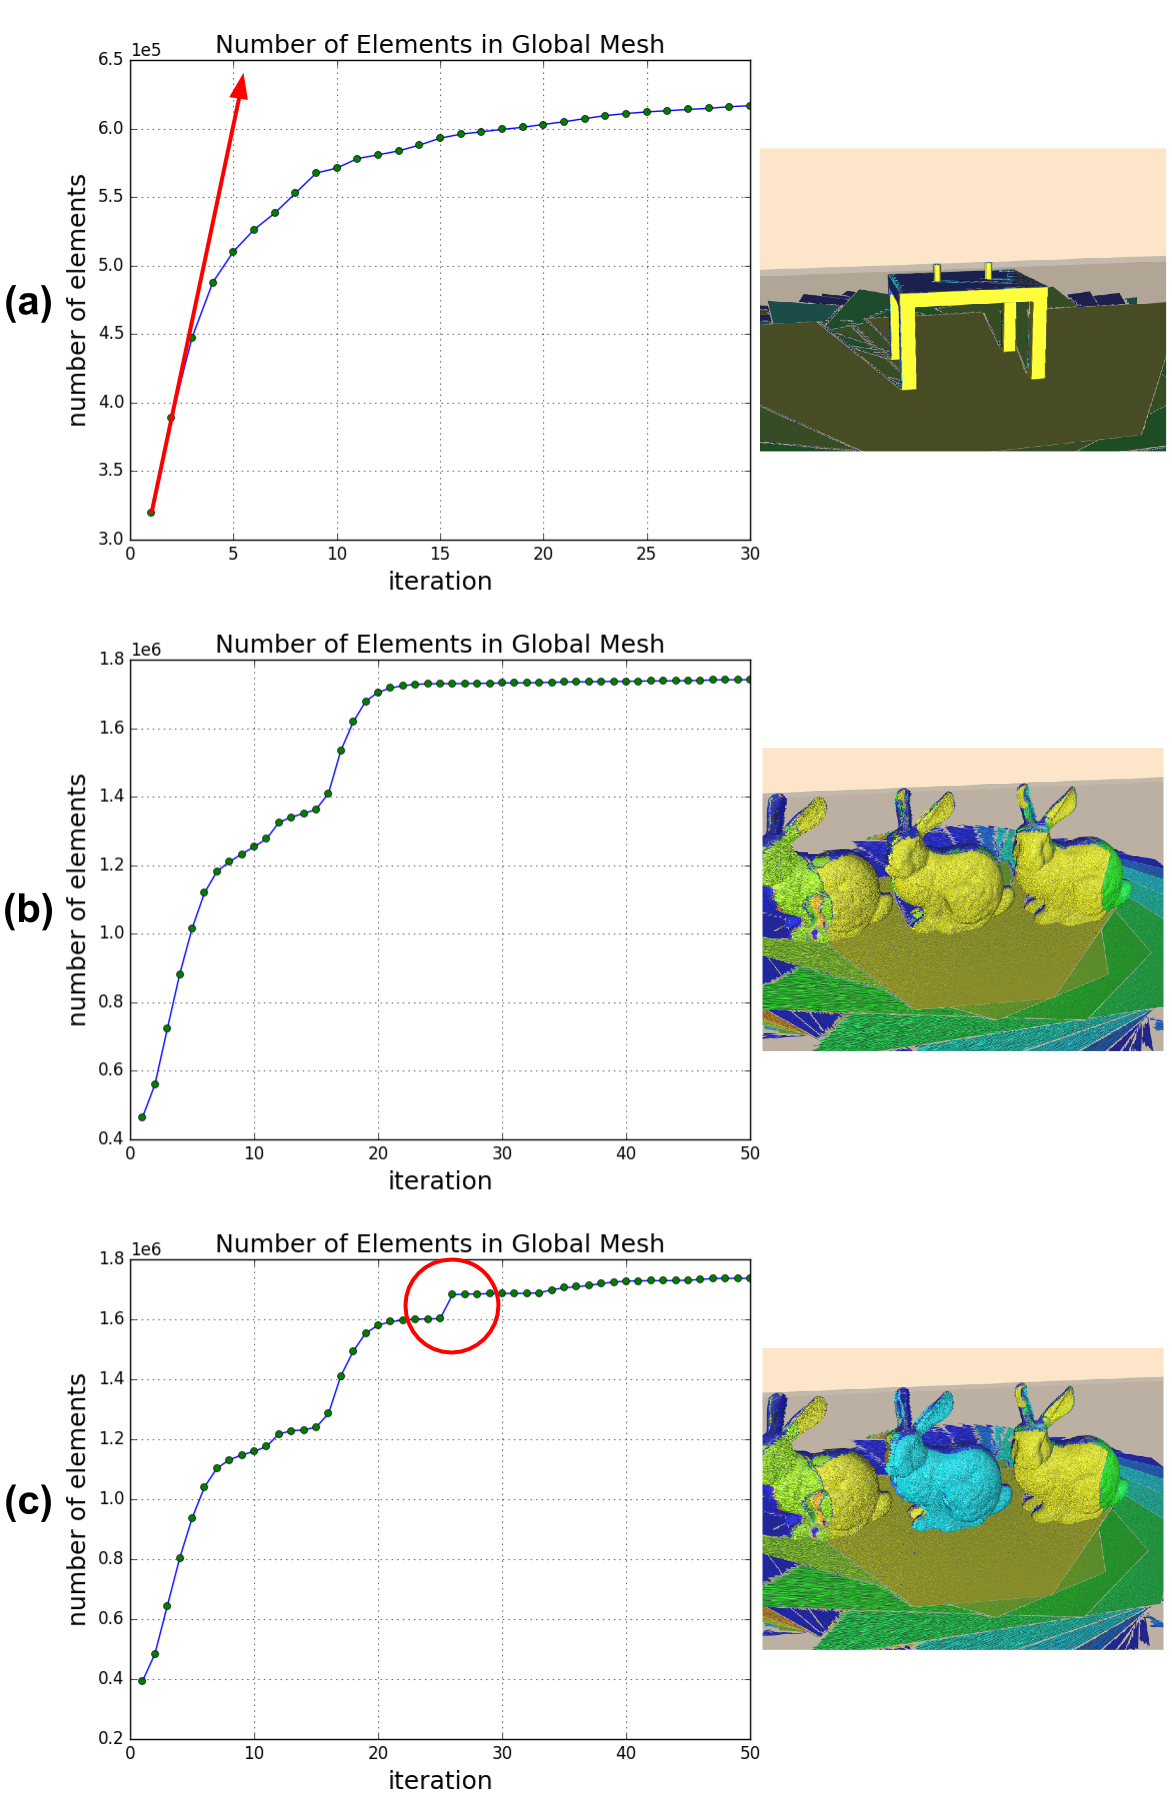
\includegraphics[width=0.48\textwidth]{figures/diagram_run123_gm.png}
\caption{Global mesh results. Top: Run1. Middle: Run2. Bottom: Run3}
\label{fig:gm}
\end{figure}

% Results of the runs
% Definitely talk about how adding a bunny worked well

\section{Results} \label{sec:results}

% discuss difficulty with noise
% how to expand to deal with object deletion

\bibliographystyle{IEEEtran}
\bibliography{bibliography}

\end{document}
